\documentclass{beamer}
\usepackage[utf8]{inputenc}
\usepackage[english]{babel}
\usecolortheme{whale}
\usepackage{pgf,tikz,pgfplots}
\pgfplotsset{compat=1.15}
\usepackage{mathrsfs}
\usetikzlibrary{arrows}
\usepackage{graphicx}

\newcommand{\R}{\mathbb{R}}
\newcommand{\Z}{\mathbb{Z}}

% set font encoding for PDFLaTeX, XeLaTeX, or LuaTeX
\usepackage{ifxetex,ifluatex}
\newif\ifxetexorluatex
\ifxetex
  \xetexorluatextrue
\else
  \ifluatex
    \xetexorluatextrue
  \else
    \xetexorluatexfalse
  \fi
\fi

\ifxetexorluatex
  \usepackage{fontspec}
\else
  \usepackage[T1]{fontenc}
  \usepackage[utf8]{inputenc}
  \usepackage{lmodern}
\fi

\usepackage{hyperref}

\title{Motores y sentimientos:\\ Análisis topológico de señales acústicas}
\author{Javier Aguilar Martín}
\institute{Universidad de Sevilla}
% Enable SageTeX to run SageMath code right inside this LaTeX file.
% http://mirrors.ctan.org/macros/latex/contrib/sagetex/sagetexpackage.pdf
% \usepackage{sagetex}

\begin{document}
\frame{\titlepage}

\begin{frame}
\frametitle{Problemas}

\begin{block}{Problema 1}
Determinar si un motor es bueno o defectuoso a partir del sonido que emiten.
\end{block}\pause

\begin{block}{Problema 2}
Determinar el estado de ánimo de una persona a partir de su voz.
\end{block}\pause
\vspace{0.5cm}

\begin{itemize}
\item Ambos consisten en clasificar distintos tipos de señales acústicas.
\end{itemize}

\end{frame}




\begin{frame}
\frametitle{Datos de entrada}
Recibimos los valores que toma una señal $f:\R^n\to\R$ en un conjunto finito $S\subset \R^n$.

\begin{itemize}
\item<2-> La primera coordenada de los puntos representa el tiempo.
\item<3-> Se perturbará ligeramente $f$ para que sea inyectiva (necesario para la filtración).
\item<4-> Las señales se pueden considerar como funciones $f:\R^n\to c\Z$, donde $c$ es la \emph{precisión} del aparato de medida.
\item<5-> Por motivos de eficiencia se puede tomar un subconjunto más pequeño $S'\subset S$.
\end{itemize}
\end{frame}



\begin{frame}
\frametitle{Complejo simplicial}

Sea $K$ el complejo simplicial construido de la siguiente forma:
\begin{itemize}
\item<2-> Tomamos $S$ como conjunto de vértices.
\item<3-> Ordenamos los puntos de $S$ según la primera coordenada.
\item<4-> Añadimos una arista por cada par de vértices consecutivos.
\end{itemize}\pause

\only<5>{\begin{block}{Nota}
El complejo simplicial aproxima $f$ mediante una función lineal a trozos. 
\end{block}}

\end{frame}



\begin{frame}
\frametitle{Filtración}
\begin{block}{Lower star filtration}
\begin{itemize}
\item<2-> Sea $\{u_1,\dots, u_p\}=S$ y consideremos los valores $f(u_1),\dots, f(u_p)$.
\item<3-> Los valores de $f$ se pueden ordenar incrementalmente: $f(u_{i_1})<\cdots<f(u_{i_p})$. 
\item<4-> La filtración \emph{lower star} de $K$ está dada por los subcomplejos
\[
K_j=\{\sigma\in K\mid \forall v\leq\sigma, f(v)\leq f(u_{i_j})\}.
\]
\end{itemize}

\end{block}

\end{frame}



\begin{frame}
\begin{block}{Ejemplo}
\begin{figure}
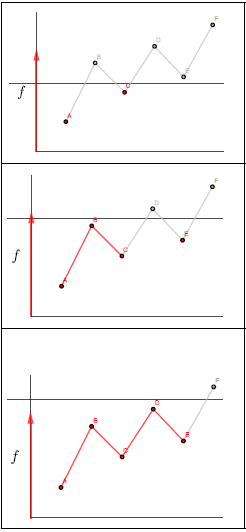
\includegraphics[scale=0.55]{low}
\end{figure}
\end{block}
\end{frame}





\begin{frame}


\frametitle{Entropía}

\begin{block}{Motores}
\begin{itemize}
\item<2-> Se probaron 46 motores.
\item<3-> Las señales se midieron a un ritmo de 50kHz hasta un total de 180000 puntos (359999 aristas).
\item<4-> La precisión de la máquina es $c=1.4386\cdot 10^{-14}$.
\item<5-> Los motores \textbf{buenos} presentan una entropía media de $H=0.6647$ con desviación típica $0.0668$. Los motores \textbf{malos} presentan una entropía media de $H=0.8001$ y desviación típica $0.0711$.

\end{itemize}

\end{block}

\end{frame}




\begin{frame}
\frametitle{Entropía}
\begin{figure}[h!]
\centering
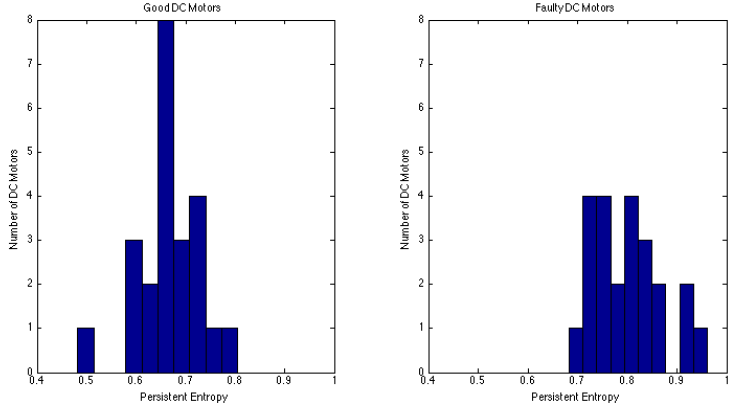
\includegraphics[scale=0.5]{motors}

La precisión óptima se alcanza fijando la barrera en $H=0.7211$, obteniendo una precisión del $89\%$. 
\end{figure}
\end{frame}


\begin{frame}
\frametitle{Entropía}
\begin{block}{Estados de ánimo}
\begin{itemize}
\item<2-> Emociones a identificar:

neutral, calma, felicidad, tristeza, enfado, miedo, asco y sorpresa
\item<3-> 24 actores interpretando 60 audios con diferentes emociones e intensidades: 4 audios para la neutral y 8 para cada una de las demás (en total, 1440 audios).
\item<4-> La clasificación se hace con ayuda de support-vector machines (SVM).
\end{itemize}
\end{block}
\end{frame}

\begin{frame}
\frametitle{Entropía}
\begin{figure}
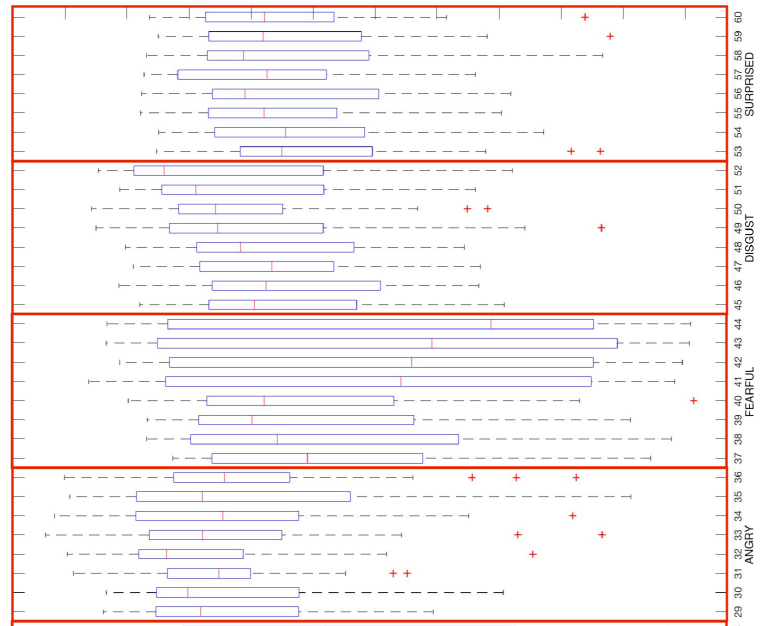
\includegraphics[scale=0.5]{emo1}
\end{figure}
\end{frame}

\begin{frame}
\frametitle{Entropía}
\begin{figure}
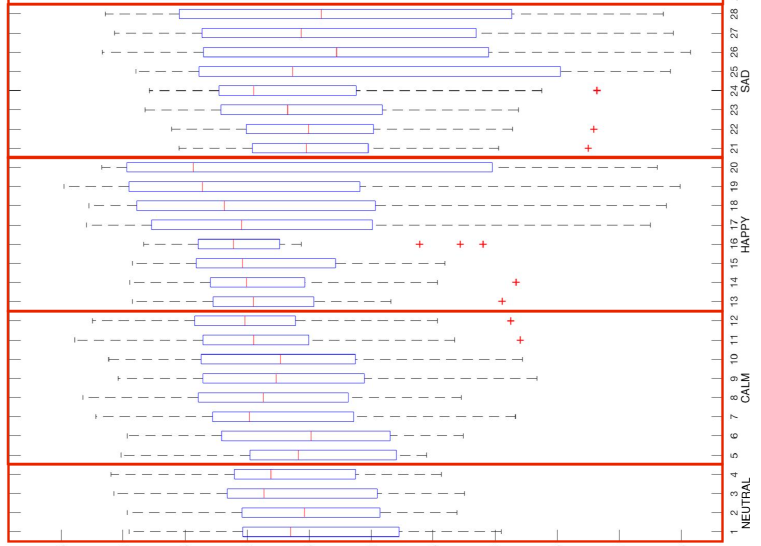
\includegraphics[scale=0.5]{emo2}
\end{figure}

\end{frame}

\begin{frame}
\frametitle{Resultados}
\begin{itemize}
\item<1-> Se observa gran variabilidad entre personas y solapamiento entre emociones. Aun así es posible detectar pares de emociones.
\item<2-> Tabla de precisión por pares
\begin{figure}
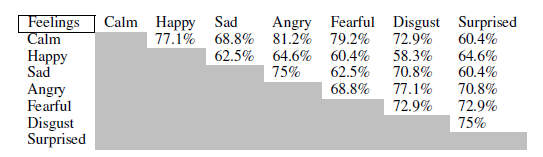
\includegraphics[scale=0.7]{precision}
\end{figure}
\end{itemize}
\begin{figure}
%
\includegraphics[scale=0.6]{close}
\end{figure}
\end{frame}

\begin{frame}
\frametitle{Resultados}
\begin{itemize}
\item<1-> Se observa más correlación entre actores del mismo sexo.
\begin{figure}
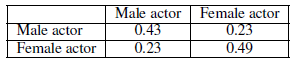
\includegraphics[scale=0.8]{sexos}
\end{figure}
\end{itemize}
\end{frame}


\begin{frame}
\frametitle{Resultados}

\begin{block}{Modificaciones del experimento}
\begin{itemize}
\item<1-> Cada punto del conjunto de datos pasa tener 24 coordenadas que representan la entropía persistente de la misma emoción interpretada por los 24 actores:
\begin{itemize}
\item Se consigue una precisión superior al 90\%.
\end{itemize}
\item<2-> Cada punto es un vector de 8 coordenadas correspondientes a la entropía persistente de cada emoción representada por el mismo actor:
\begin{itemize}
\item Precisión del 71\% pero más fácil de realizar que el anterior.
\end{itemize}
\item<3-> Se propone combinar los experimentos con análisis gesticulares de los rostros de los actores.
\end{itemize}
\end{block}


\end{frame}





\begin{frame}
\begin{center}


\begin{Huge}
Gracias
\end{Huge}
\end{center}
\end{frame}




\end{document}
